\documentclass[]{article}
\usepackage{lmodern}
\usepackage{amssymb,amsmath}
\usepackage{ifxetex,ifluatex}
\usepackage{fixltx2e} % provides \textsubscript
\ifnum 0\ifxetex 1\fi\ifluatex 1\fi=0 % if pdftex
  \usepackage[T1]{fontenc}
  \usepackage[utf8]{inputenc}
\else % if luatex or xelatex
  \ifxetex
    \usepackage{mathspec}
  \else
    \usepackage{fontspec}
  \fi
  \defaultfontfeatures{Ligatures=TeX,Scale=MatchLowercase}
\fi
% use upquote if available, for straight quotes in verbatim environments
\IfFileExists{upquote.sty}{\usepackage{upquote}}{}
% use microtype if available
\IfFileExists{microtype.sty}{%
\usepackage{microtype}
\UseMicrotypeSet[protrusion]{basicmath} % disable protrusion for tt fonts
}{}
\usepackage[margin=1in]{geometry}
\usepackage{hyperref}
\hypersetup{unicode=true,
            pdftitle={Testosterone, diversity, and group project performance},
            pdfauthor={Cathy Su},
            pdfborder={0 0 0},
            breaklinks=true}
\urlstyle{same}  % don't use monospace font for urls
\usepackage{graphicx,grffile}
\makeatletter
\def\maxwidth{\ifdim\Gin@nat@width>\linewidth\linewidth\else\Gin@nat@width\fi}
\def\maxheight{\ifdim\Gin@nat@height>\textheight\textheight\else\Gin@nat@height\fi}
\makeatother
% Scale images if necessary, so that they will not overflow the page
% margins by default, and it is still possible to overwrite the defaults
% using explicit options in \includegraphics[width, height, ...]{}
\setkeys{Gin}{width=\maxwidth,height=\maxheight,keepaspectratio}
\IfFileExists{parskip.sty}{%
\usepackage{parskip}
}{% else
\setlength{\parindent}{0pt}
\setlength{\parskip}{6pt plus 2pt minus 1pt}
}
\setlength{\emergencystretch}{3em}  % prevent overfull lines
\providecommand{\tightlist}{%
  \setlength{\itemsep}{0pt}\setlength{\parskip}{0pt}}
\setcounter{secnumdepth}{0}
% Redefines (sub)paragraphs to behave more like sections
\ifx\paragraph\undefined\else
\let\oldparagraph\paragraph
\renewcommand{\paragraph}[1]{\oldparagraph{#1}\mbox{}}
\fi
\ifx\subparagraph\undefined\else
\let\oldsubparagraph\subparagraph
\renewcommand{\subparagraph}[1]{\oldsubparagraph{#1}\mbox{}}
\fi

%%% Use protect on footnotes to avoid problems with footnotes in titles
\let\rmarkdownfootnote\footnote%
\def\footnote{\protect\rmarkdownfootnote}

%%% Change title format to be more compact
\usepackage{titling}

% Create subtitle command for use in maketitle
\providecommand{\subtitle}[1]{
  \posttitle{
    \begin{center}\large#1\end{center}
    }
}

\setlength{\droptitle}{-2em}

  \title{Testosterone, diversity, and group project performance}
    \pretitle{\vspace{\droptitle}\centering\huge}
  \posttitle{\par}
    \author{Cathy Su}
    \preauthor{\centering\large\emph}
  \postauthor{\par}
      \predate{\centering\large\emph}
  \postdate{\par}
    \date{27/10/2019}


\begin{document}
\maketitle

\subsection{Executive Summary}\label{executive-summary}

In this report, we analyze a demographic data set collected by
\emph{(Akinola et al. 2018)} and explore the relationship between a set
of variables that contribute to group performance on a competetive task.
The data comprises individual level and group level statistics collected
from groups of MBA students completing a 7-day group project. We use
exploratory data analysis and regression models to mainly explore how
\textbf{diversity, testosterone and cortisol} levels affect
\textbf{final.performance}. We hypothesized that high levels of
testosterone and cortisol would both prevent group cooperation leading
to low performance. Therefore we expected to see similar effects of
these two hormones and their interaction with diversity score upon
performance.

We first performed variable selection with best subsets and cross
validation to exclude variables with negligible effect on the response
of performance score. Based upon this we selected eight covariates
including diversity, testosterone and cortisol. Mean and variance of
ages was not found to be a significant explanatory variable, but the
proportion of females in teh group was. We fit regression models both
with and without cortisol related terms. We found that when not
accounting for cortisol, diversity has a positive effect on performance,
but only if group-level testosterone is low. This resembles the results
presented by the original study. To resolve the results of these two
different models, we then used cross validation to select the model with
the best performance by best subset regression, which contains both
hormones as well as their interaction effects with diversity.

\subsection{Introduction}\label{introduction}

Diversity and conflict are considered important factors which influence
how well we work in groups (Knippenberg and Schippers 2007). As the
working world becomes more connected across the globe and thus the
diversity of organizational groups increases, it is important to
characterize the effect of diversity on group performance. Previous work
by (Akinola et al. 2018) suggests that both diversity and group hormone
levels will influence how well groups perform on a competetive task. In
their study, they considered levels of the two hormones testosterone and
cortisol. Testosterone is involved in dominance and competition related
behaviour in individuals and is produced at a higher level in males than
females, while cortisol is a hormone released during physical and
psychological stress (P. H. Mehta and Prasad 2015). For healthy males
between 19 to 40 years, normal testosterone is known to fall within the
15.4 to 13 nmol/L range (Kelsey et al. 2014).

In their work, (Akinola et al. 2018) collected both demographic data and
hormone measurements from 370 MBA students organized into 74 groups who
partcipated in a competitive week long project where their goal was to
outperform other groups. There were 370 individuals randomly organized
into 74 groups. Based on their demographic and hormone measurement data,
the authors concluded that diversity is beneficial for performance, but
only if group-level testosterone is low; and diversity has a negative
effect on performance if group-level testosterone is high. However, the
authors did not mention analyzing cortisol even though cortisol levels
is suggested to have an effect testosterone's role in status-relevant
behavior (P. H. Mehta and Prasad 2015).

To validate the author's hypothesis and additionally examine the
specific role of cortisol, we are using the (Akinola et al. 2018)
dataset which has been processed by
\href{http://rosmarus.refsmmat.com/datasets/datasets/hormone-diversity/}{Nifty
Datasets} into separate individual level and group level datasets. Based
on the preamble, we hypothesized that the effects of testosterone and
diversity on performance are mediated by their opposite effects on
`cooperation' (not directly measured) in the group. Furthermore cortisol
levels largely unevaluated by the study may influence performance
through affecting group `stress' (not directly measured). Putting this
together with the measured variables, we illustrate our hypotheses about
the data in Figure \ref{fig:cause}. Following from this diagram, we
calculated the group level proportion of females, average age and
variance of age.

Since there were many covariates to consider, we first performed
variable selection with best subsets to exclude variables with
negligible effect on the response of performance score. With this we
were able to focus upon 8 variables of interest which included two terms
describing interaction of each hormone measurement with diversity score.
By fitting a linear model including the selected covariates, we verified
teh authors' finding that when group diversity is low, testosterone is
positively correlated with group performance and when group diversity is
high, testosterone is negatively correlated with group performance. We
also found that cortisol and its interaction with diversity score were
not found to be significant explanatory variables of final performance
when we included them into the model.

\begin{figure}
\centering
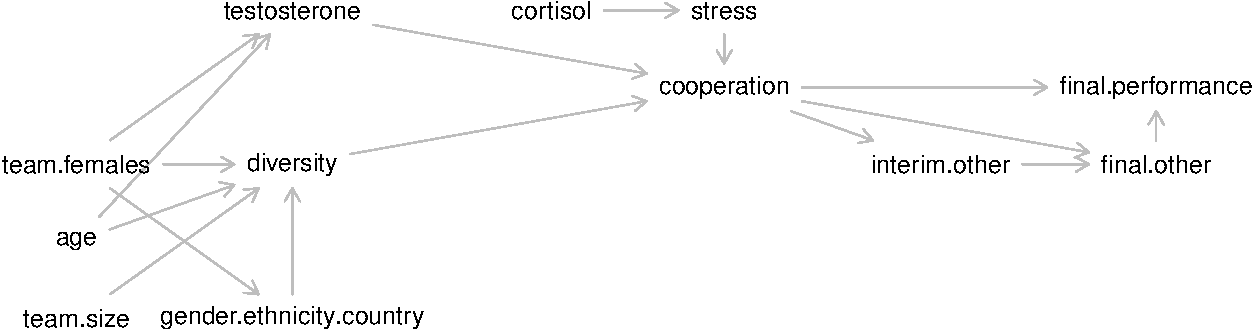
\includegraphics{19_10_27_hw7_q1_files/figure-latex/causal-1.pdf}
\caption{\label{fig:cause}Causal diagram illustrates hypothesized
relationships of experimental variables involved in relationship between
testosterone and final group performance.}
\end{figure}

\subsection{Methods}\label{methods}

\subsubsection{Calculation of group level variables and removal of
outliers}\label{calculation-of-group-level-variables-and-removal-of-outliers}

We are interested in doing our analysis at the group level therefore we
needed to aggregate the individual level data. We saw there were
\textless{}10 individuals with partly missing data. Since we are trying
to look at team level performance, we did not remove any individuals.
For these individuals, not everything was missing so we calculated group
average measurements, e.g.~average hormone measurements, from other
members. Additionally, we have calculated group diversity score as the
number of unique gender-ethnicity-country combinations present in the
group. Lastly we calculate proportion of females in the group as the
number of females divided by group size. We then examined whether there
were any groups with outlier measurements for the key variables:
diversity score, hormone measurements and team performance.

\subsection{Exploratory Data Analysis \& Data
Summary}\label{exploratory-data-analysis-data-summary}

After aggregating data to the group level, we checked the distributions
of all of the variables (not shown). Only measurements in the `interim'
variables are missing. Given that it's unclear how the multiple interim
measurements may relate to the final score and they contain many missing
values, we removed these variables. However, the limitation is that we
may be very dependent upon a single measure of performance, which would
be the single score assigned to the variable ``final.performance''.

\subsubsection{Distribution of hormone levels across individuals and
groups}\label{distribution-of-hormone-levels-across-individuals-and-groups}

It was clear when for both hormone levels that the log transformed
values were distributed with less skew across teams than the raw values
and have fewer outlier values. This is preferable so we chose like the
authors to use averaged log testosterone per group. Figure
\ref{fig:test} shows the distribtuions for testosterone but for cortisol
the difference is similar.

\begin{figure}
\centering
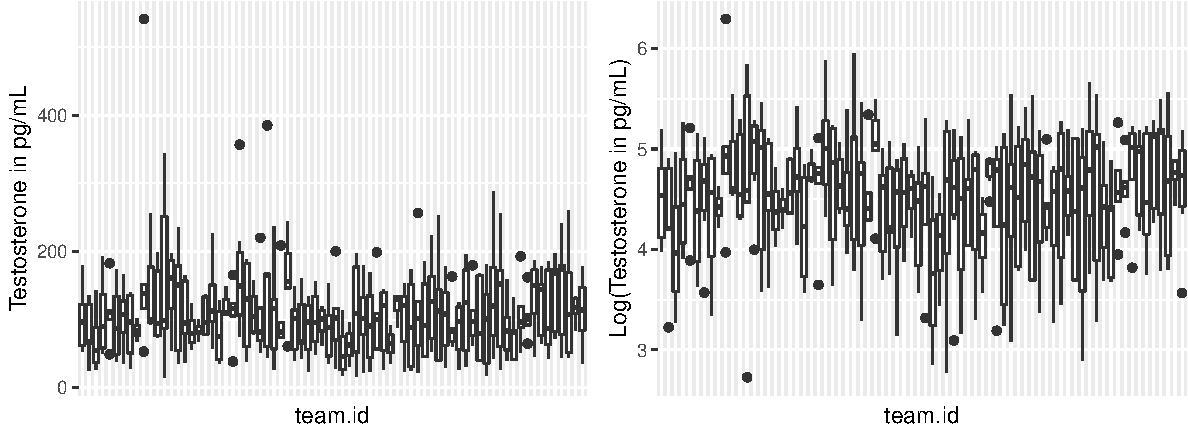
\includegraphics{19_10_27_hw7_q1_files/figure-latex/test-1.pdf}
\caption{\label{fig:test}Distributions of testosterone and log
testosterone levels in each team.}
\end{figure}

\subsubsection{Incorporation of age and
gender}\label{incorporation-of-age-and-gender}

Both age and gender were included in the results of the original
manuscript. Based upon our causal graph, both can have an influence on
final performance through influencing testosterone levels or through
influencing diversity. We know we need to study their impact on
teamwork, therefore it makes sense to look at the proportion of females
in the group and the variance of age in the group which are measures of
diversity. We also know that hormone levels depend upon age, therefore
we also calculate average age in the group.

\subsubsection{Univariate and pairwise distributions of group level
variables}\label{univariate-and-pairwise-distributions-of-group-level-variables}

The univariate distributions of the group level variables is given
across the diagonal in Figure \ref{fig:pairs}. We see that in
particular, our diversity score appears bimodal. Although our score is
calculated differently, (Akinola et al. 2018) classified diversity score
into two bins in their faultline analysis suggesting that our diversity
score may behave similarly.

In the same figure we have the pairwise comparisons of the important
variables as well. In the upper diagonal, the Pearson correlation
coefficients (upper right half) between important variables are
described with their significance.

Based upon the summary statistics and the distributions seen in Figure
\ref{fig:pairs}, we noted the following outlier teams:

\begin{itemize}
\tightlist
\item
  we likely do not need to discard variables based on collinearity.
\item
  teams 65, 92 and 101 had very low final performance (below a score of
  -2).
\item
  team 64 had very low log testosterone.
\item
  team 39 was the only one with no female members.
\end{itemize}

However, we did not remove these outliers at the outset because we
actually don't have many teams to fit the model on and the outliers lay
within wo standard deviations of the mean of each variable in question.

\begin{figure}
\centering
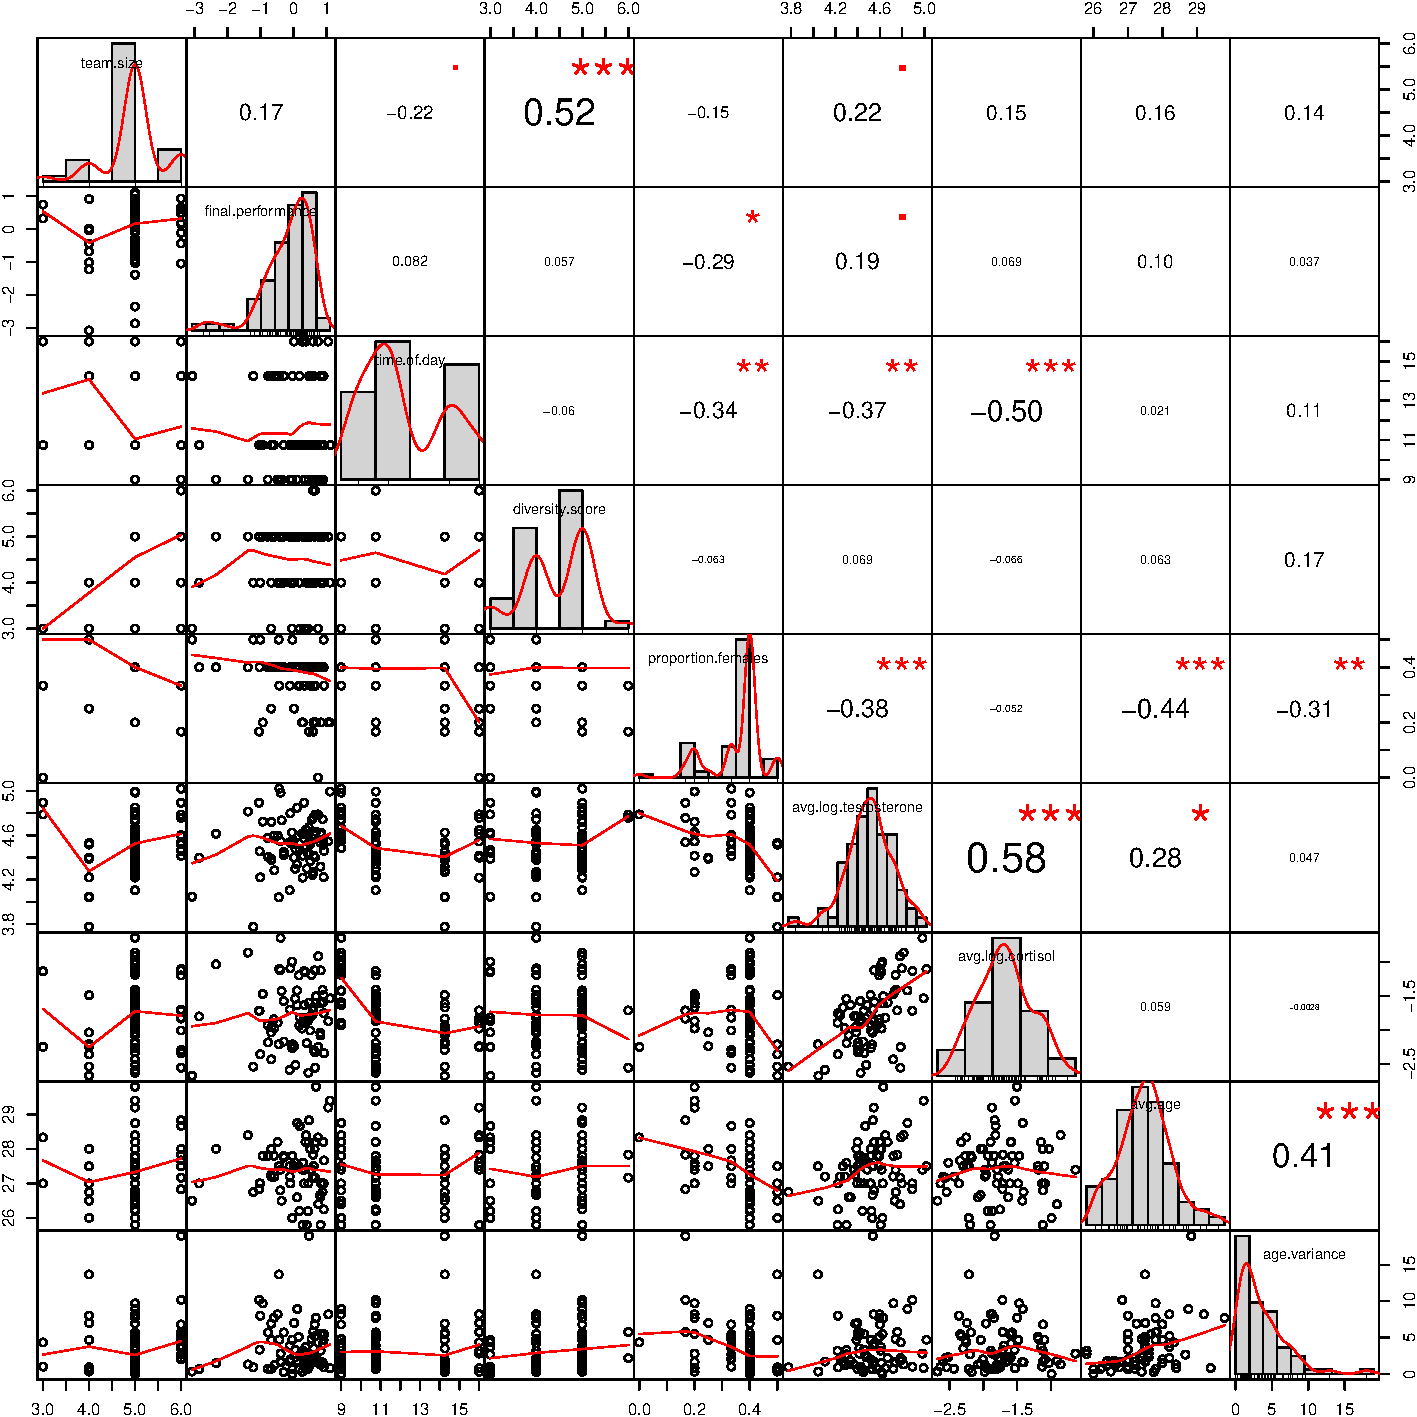
\includegraphics{19_10_27_hw7_q1_files/figure-latex/dists-1.pdf}
\caption{\label{fig:pairs}Pairwise correlations of important variables
including their Pearson correlation coefficient. Significant
correlations are marked by the corresponding number of astericks.}
\end{figure}

\subsection{Results}\label{results}

\subsubsection{Selecting the variables with non-negligible
effect}\label{selecting-the-variables-with-non-negligible-effect}

Out of the variables that we had considered in Figure \ref{fig:pairs},
to build models we first performed variable selection to exclude those
without large effects. We included the interaction terms between
diversity score and each of the hormones, which are interpretable
interaction terms that we need to consider to answer the substantive
questions. First we picked how many terms we should have in the best
predictive linear model by using 10-fold cross validation and plotted
the mean squared error in Figure \ref{fig:cv}. This analysis shows
validation error is lowest around 8 terms.

\begin{figure}
\centering
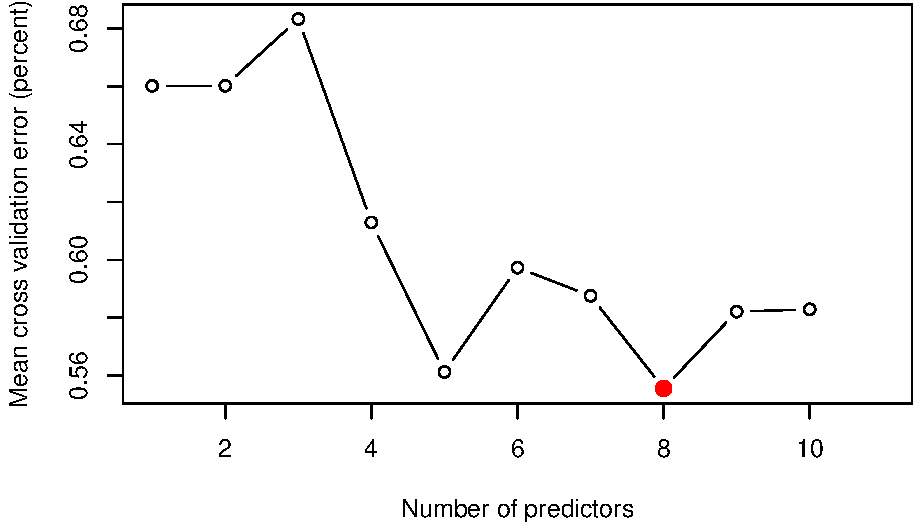
\includegraphics{19_10_27_hw7_q1_files/figure-latex/cv-1.pdf}
\caption{\label{fig:cv} Cross validation error for each number of
predictors}
\end{figure}

Based on this we used best subset selection on the full data set in
order to obtain the best 8-predictor model. The variables and
coefficients selected by the model are given in Table 1. While the
coefficients of the predictive model are not necessarily useful for
explaining the final group performance, the predictive model includes
only variables with non-negligible effect. This suggests to us that age
variance for example is not a useful explanatory variable, and we
discarded these extra variables.

\begin{table}

\caption{\label{tab:unnamed-chunk-2}Variables selected for 8-variable model found by best subsets regression}
\centering
\begin{tabular}[t]{l|r}
\hline
  & x\\
\hline
(Intercept) & -37.9400016\\
\hline
team.size & 0.3315728\\
\hline
time.of.day & 0.0561873\\
\hline
diversity.score & 7.7455914\\
\hline
proportion.females & -1.0946513\\
\hline
avg.log.testosterone & 8.6333483\\
\hline
avg.log.cortisol & 1.6009332\\
\hline
diversity.score:avg.log.testosterone & -1.8703343\\
\hline
diversity.score:avg.log.cortisol & -0.3799276\\
\hline
\end{tabular}
\end{table}

\subsubsection{Effect of group diversity on relationship between
testosterone and
performance}\label{effect-of-group-diversity-on-relationship-between-testosterone-and-performance}

The results discussed by the original study (Akinola et al. 2018)
suggest that when group diversity was low, group testosterone
significantly positively predicted performance at p \textless{} .01 when
group diversity was relatively high, group testosterone significantly
negatively predicted performance p \textless{}0.01. However they were
not considering cortisol at the time. Given this we fit a model of final
performance using all of the variables chosen from Table 1 except those
terms which included cortisol. The coefficients which we found are
displayed in Table 2.

\begin{table}[!htbp] \centering 
  \caption{Terms included in model of testosterone and performance} 
  \label{tab:regression} 
\small 
\begin{tabular}{@{\extracolsep{1pt}}lc} 
\\[-1.8ex]\hline 
\hline \\[-1.8ex] 
 & \multicolumn{1}{c}{\textit{Dependent variable:}} \\ 
\cline{2-2} 
\\[-1.8ex] & final.performance \\ 
 & model 1 \\ 
\hline \\[-1.8ex] 
 Constant & $-$49.030$^{***}$ (11.389) \\ 
  team.size & 0.387$^{**}$ (0.176) \\ 
  time.of.day & 0.061 (0.048) \\ 
  diversity.score & 10.176$^{***}$ (2.432) \\ 
  proportion.females & $-$0.842 (1.203) \\ 
  avg.log.testosterone & 10.360$^{***}$ (2.402) \\ 
  diversity.score:avg.log.testosterone & $-$2.257$^{***}$ (0.536) \\ 
 \hline \\[-1.8ex] 
Observations & 74 \\ 
R$^{2}$ & 0.298 \\ 
Adjusted R$^{2}$ & 0.235 \\ 
Residual Std. Error & 0.733 (df = 67) \\ 
F Statistic & 4.738$^{***}$ (df = 6; 67) \\ 
\hline 
\hline \\[-1.8ex] 
\end{tabular} 
\end{table}

We verified that this model could provide a good fit to the data by
looking at the diagnostic plots in Figure \ref{fig:x}. We found that
there were two outliers with low residuals (marked 66 and 59) in the
plot of residuals vs.~fitted and the normal QQ-plot, but these were not
highly influential points as measured by Cook's distance which is shown
in the Residuals vs.~Leverage plot.

\begin{figure}
\centering
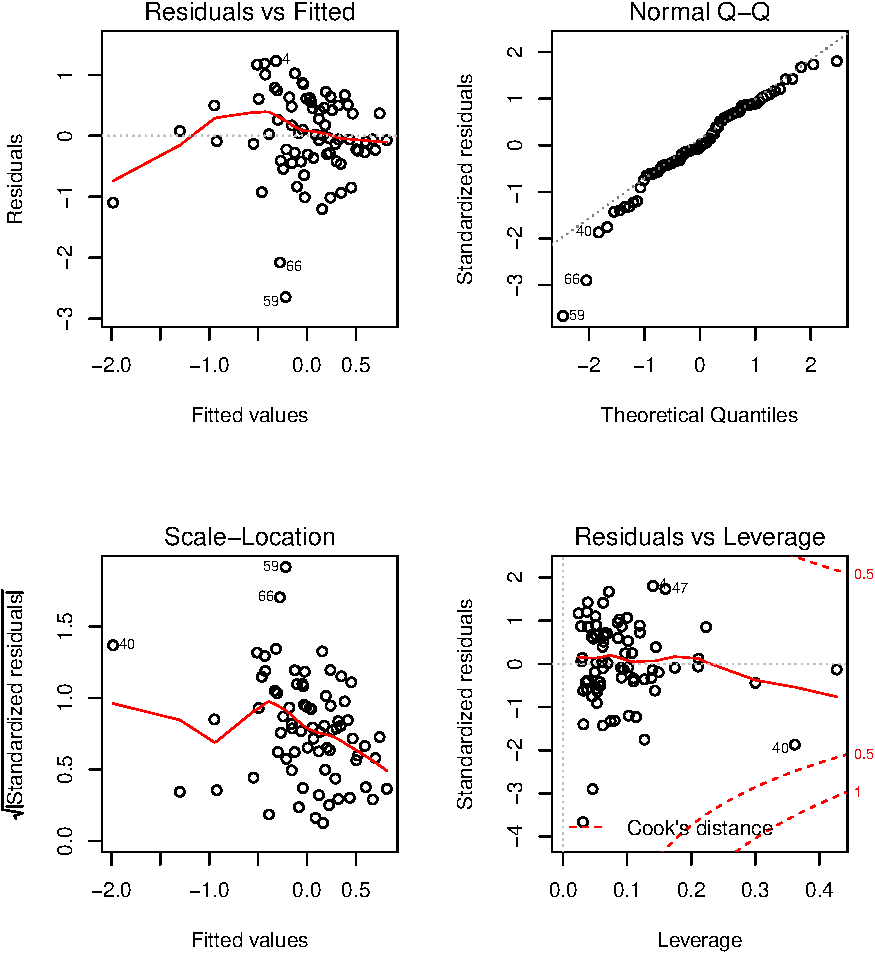
\includegraphics{19_10_27_hw7_q1_files/figure-latex/unnamed-chunk-3-1.pdf}
\caption{\label{fig:x} Residuals for Model from Table 2}
\end{figure}

In this model, the interaction term diversity.score:avg.log.testosterone
is indeed significant (coefficient = -2.2574, p \textless{} 0.001). The
negative sign of the coefficient implies that there is an opposite
effect on performance from each of the two predictors diversity and
testosterone. This is better illustrated in Figure \ref{fig:int} where
we can see that when diversity is low at 3 units, group testosterone
positively correlates with performance whereas when diversity is high at
6 units testosterone negatively correlates with performance. This
suggests that we have verified the findings of the authors.

\begin{figure}
\centering
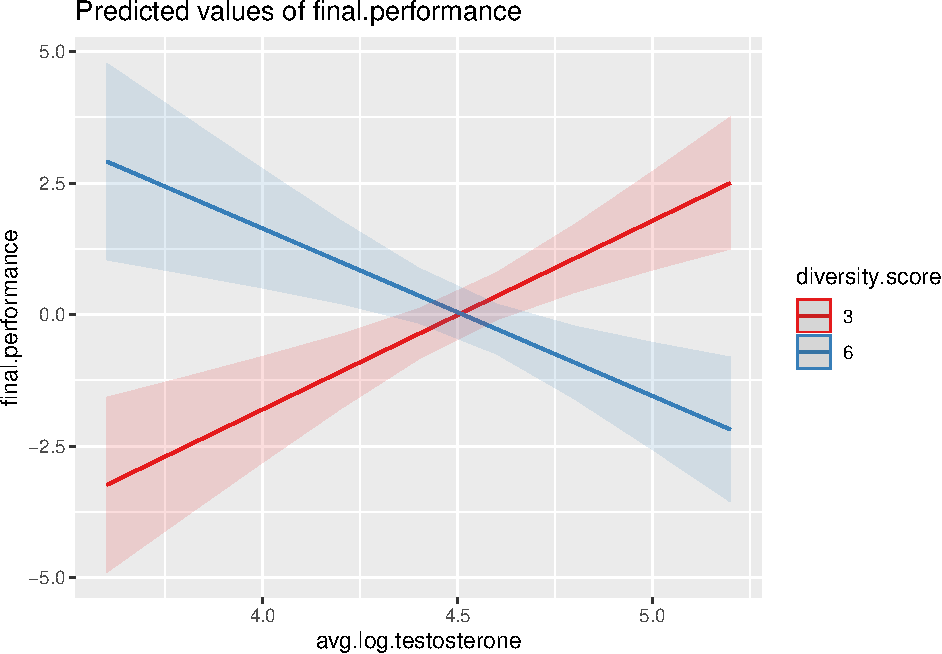
\includegraphics{19_10_27_hw7_q1_files/figure-latex/unnamed-chunk-4-1.pdf}
\caption{\label{fig:int}Interaction between diversity and performance.
The plot suggests that as the authors found, group diversity mediates
teh effect of testosterone on performance.}
\end{figure}

\subsubsection{Effect of cortisol on relationship between diversity and
performance}\label{effect-of-cortisol-on-relationship-between-diversity-and-performance}

Our EDA and variable selection had shown us that cortisol might be
useful to include in our explanatory model of performance and so we
additionally tested a model which includes cortisol levels and their
interaction with diversity (Table 3). However we found that in this
model, neither cortisol nor its interaction with diversity are found to
have a significant effect at p \textless{} 0.05.

\begin{table}[!htbp] \centering 
  \caption{Terms included in model of cortisol, testosterone and performance} 
  \label{tab:regression} 
\small 
\begin{tabular}{@{\extracolsep{1pt}}lc} 
\\[-1.8ex]\hline 
\hline \\[-1.8ex] 
 & \multicolumn{1}{c}{\textit{Dependent variable:}} \\ 
\cline{2-2} 
\\[-1.8ex] & final.performance \\ 
 & model 3 \\ 
\hline \\[-1.8ex] 
 Constant & $-$37.995$^{**}$ (15.781) \\ 
  team.size & 0.336$^{*}$ (0.187) \\ 
  time.of.day & 0.055 (0.051) \\ 
  diversity.score & 7.881$^{**}$ (3.250) \\ 
  proportion.females & $-$1.098 (1.338) \\ 
  avg.log.testosterone & 8.787$^{***}$ (3.049) \\ 
  avg.log.cortisol & 1.553 (1.355) \\ 
  avg.age & $-$0.027 (0.127) \\ 
  age.variance & 0.007 (0.030) \\ 
  diversity.score:avg.log.cortisol & $-$0.372 (0.287) \\ 
  diversity.score:avg.log.testosterone & $-$1.898$^{***}$ (0.655) \\ 
 \hline \\[-1.8ex] 
Observations & 74 \\ 
R$^{2}$ & 0.322 \\ 
Adjusted R$^{2}$ & 0.214 \\ 
Residual Std. Error & 0.743 (df = 63) \\ 
F Statistic & 2.992$^{***}$ (df = 10; 63) \\ 
\hline 
\hline \\[-1.8ex] 
\end{tabular} 
\end{table}

Again we verified that this model could provide a good fit to the data
by looking at the diagnostic plots in Figure \ref{fig:y}. The same two
outliers with low residuals found in the model of testosterone and
performance were present here (marked 66 and 59) but these were these
were again not highly influential points as measured by Cook's distance
which is shown in the Residuals vs.~Leverage plot. We also note that the
value of the adjusted R squared in this model is about the same as in
the model without cortisol terms (0.214 vs 0.235 respectively)
suggesting the data may be approximately as well fit to this linear
model.

\begin{figure}
\centering
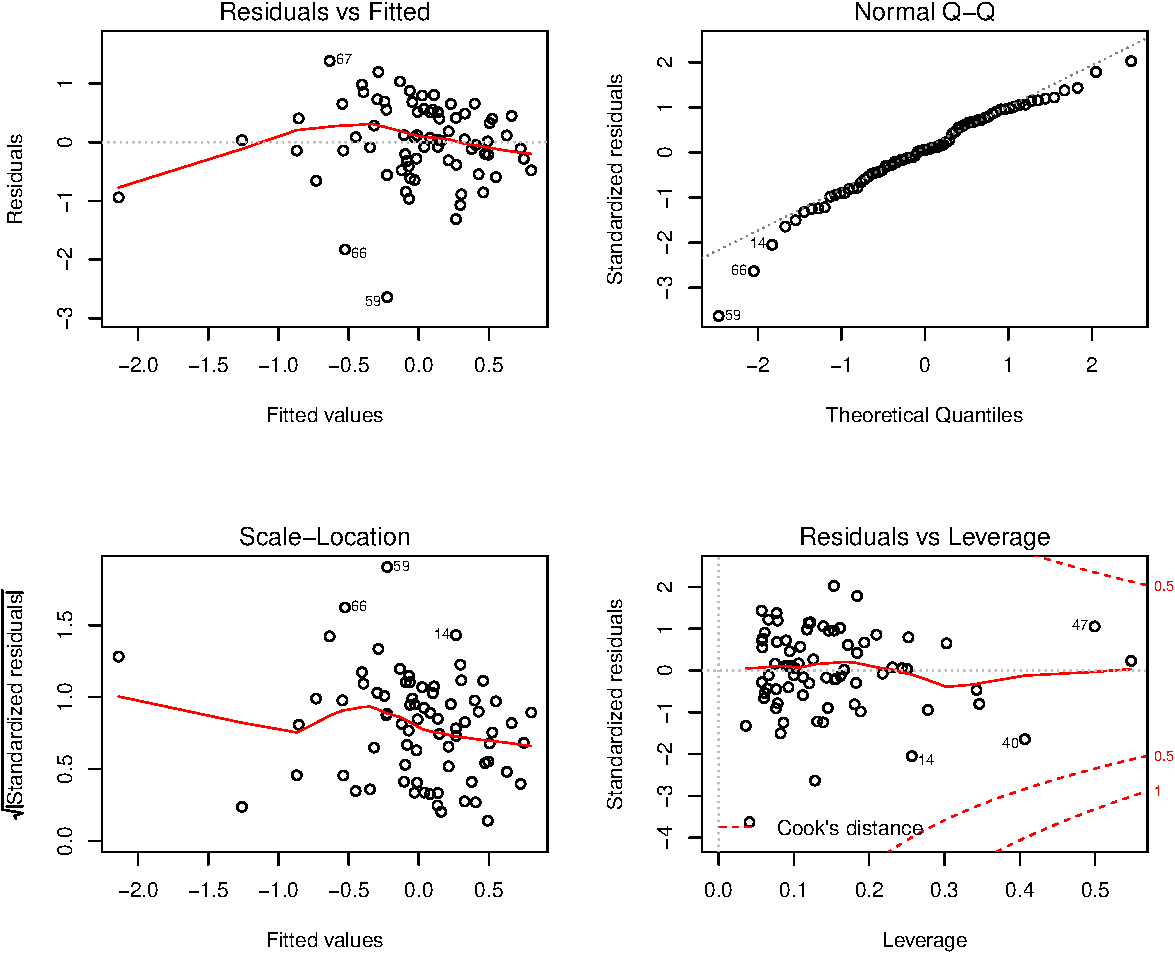
\includegraphics{19_10_27_hw7_q1_files/figure-latex/unnamed-chunk-6-1.pdf}
\caption{\label{fig:y} Residuals for Model from Table 3}
\end{figure}

In this model, the average log cortisol variable has a positive
coefficient suggesting that stressed groups have better performance.
There is a negative coefficient on the diversity.score:avg.log.cortisol
term suggesting that like with testosterone, stress changes the effect
of diversity on performance and specifically a unit increase in average
log cortisol has an antagonizing effect to a unit increase in diversity.
However the terms are not found to be significant so we will need to do
further study to determine whether cortisol has an effect on group
performance or not.

\subsubsection{Conclusion}\label{conclusion}

Here we have analyzed demographic data and hormone measurements from
groups of MBA students performing a competetive project, previously
published by (Akinola et al. 2018). We sought to investigate the
authors' hypothesis that group diversity has a testosterone-dependent
effect on group performance and also to check whether cortisol levels
had an effect on this relationship.

By building linear models and comparing the nested models with an
F-test, we have shown that when we do not account for cortisol the
interaction between diversity and testosterone has a significant
negative effect on performance (p \textless{} 0.01) implying that high
diversity and high testosterone are antagonizing factors. This agrees
with the authors' findings that diversity is beneficial for performance,
but only if group-level testosterone is low.

Additionally, we found that when we incorporate terms for cortisol and
its interaction with diversity without accounting for the interaction of
testosterone with diversity, we build a linear model where stress has a
positive effect on performance but stress and group diversity have
antagonistic effects in interaction. Additionally both hormones and
their interaction with diversity were found to be part of the best
predictive model of performance by best subset regression. This analysis
suggests that perhaps, stress has a role in group performance as well
which merits further investigation.

Although we aimed to validate conclusions from (Akinola et al. 2018)
when examining diversity and testosterone, our results have limitations
because of some differences in our methodology. Most prominently,
(Akinola et al. 2018) have used a faultline analysis to evaluate
diversity whereas we have constructed a diversity score. As well, we
have not included all of the variables that are present in the models
which they tested, such as agen. We chose to discard these variables
based upon our EDA and our reasoning about the relationship between
variables collected in the study. Lastly we cannot compare our findings
about cortisol because this was not discussed in depth in their original
analysis.

\section*{Bibliography}\label{bibliography}
\addcontentsline{toc}{section}{Bibliography}

\hypertarget{refs}{}
\hypertarget{ref-Akinola2018}{}
Akinola, Modupe, Elizabeth Page-Gould, Pranjal H. Mehta, and Zaijia Liu.
2018. ``Hormone-Diversity Fit: Collective Testosterone Moderates the
Effect of Diversity on Group Performance.'' \emph{Psychological Science}
29 (6): 859--67.
doi:\href{https://doi.org/10.1177/0956797617744282}{10.1177/0956797617744282}.

\hypertarget{ref-Kelsey2014}{}
Kelsey, Thomas W., Lucy Q. Li, Rod T. Mitchell, Ashley Whelan, Richard
A. Anderson, and W. Hamish B. Wallace. 2014. ``A Validated Age-Related
Normative Model for Male Total Testosterone Shows Increasing Variance
but No Decline after Age 40 Years.'' Edited by Bin He. \emph{PLoS ONE} 9
(10): e109346.
doi:\href{https://doi.org/10.1371/journal.pone.0109346}{10.1371/journal.pone.0109346}.

\hypertarget{ref-vanK}{}
Knippenberg, Daan van, and Michaéla C. Schippers. 2007. ``Work Group
Diversity.'' \emph{Annual Review of Psychology} 58 (1): 515--41.
doi:\href{https://doi.org/10.1146/annurev.psych.58.110405.085546}{10.1146/annurev.psych.58.110405.085546}.

\hypertarget{ref-MEHTA2015163}{}
Mehta, Pranjal H, and Smrithi Prasad. 2015. ``The Dual-Hormone
Hypothesis: A Brief Review and Future Research Agenda.'' \emph{Current
Opinion in Behavioral Sciences} 3: 163--68.
doi:\href{https://doi.org/https://doi.org/10.1016/j.cobeha.2015.04.008}{https://doi.org/10.1016/j.cobeha.2015.04.008}.


\end{document}
